\chapter{Background}
\index{Background@\emph{Background}}\label{background}%
In Section~\ref{back:phylogenetics}, I give a brief introduction to phylogenies and alignments and define basic definitions and concepts that will be used throughout my dissertation.  In Section~\ref{back:hmm}, I describe Hidden Markov Models (HMMs) and their use in alignment estimation. Finally, in Section~\ref{back:app}, I describe applications of HMMs in the realm of phylogenetic placement, metagenomic analyses, and ultra-large alignment estimation.

\section{Phylogenetics}
\emph{Phylogenetics} is the study of the evolutionary relationships between different organisms.  A typical molecular phylogenetic study begins by collecting biomolecular sequences (DNA, RNA, or amino acid sequences) from the species of interest.  The evolutionary relationship between the different characters in the sequence are inferred through an alignment.  From the alignment, a tree representing the evolutionary history between the different species are inferred.  The steps, estimating an alignment and estimating a tree, are core concepts used throughout my dissertation.  I now explain provide more background details on the alignment and the tree, and how one might go about estimating alignment and tree.

\paragraph{Tree: graphical model of evolution}\label{back:phylogenetics}
A \emph{phylogeny} is a graphical model that represents the evolutionary relationships between the different species.  One of the most common representations is using a \emph{rooted tree} - a directed acyclic graph.  Each leaf in the tree represents a species, and each internal node in the tree represents a \emph{speciation event}.  Speciation events are the process in which one species give rise to new lineages of species.  The root of the tree represents the most recent common ancestor of all the species.  Throughout my dissertation, I will refer to the leaves of the tree as species, taxa, or sequences, interchangeably.  Similarly, I refer to phylogenies as trees, though a phylogeny does not necessarily have to be tree-like, and more complicated representations such as phylogenetic networks do exist~\cite{todo}.

Figure~\ref{back:phylo_tree}(a) shows an example of a rooted phylogenetic tree.  The relationship between the different species can be inferred from the tree.  For example, species $A$ and $B$ are more closely related than $A$ and $C$ because $A$ and $B$ share a more recent common ancestor (red node) than $A$ and $C$ (blue node). The example shown is a rooted tree, i.e., the direction of evolution is known, and the root of the tree represents the most recent common ancestor (MRCA) of all the species (black node).  In general, estimating the root of the tree is very difficult as most common methods for estimating phylogenies assume time-reversibility, and under these models, it is not possible to determine which node is the ancestor and which node is the descendant.  Thus, when I discuss phylogenies, I refer to unrooted trees.

Figure~\ref{back:phylo_tree}(b) shows an unrooted version of Figure~\ref{back:phylo_tree}(a).  An unrooted tree is a \emph{binary} tree if all inner nodes have a degree of 3.  If an inner node has degree greater than 3, it is called a \emph{polytomy}.  Polytomies represent evolutionary relationships that are not resolved.  Figure~\ref{back:poly} shows an example of a tree containing a polytomy.  
%Polytomies arise when there is insufficient data to resolve the relationships between different organisms, or when rapid 
\textbf{Nam:Build polytomy figure}
\begin{figure}[htpb]
\begin{subfigure}[htpb]{\textwidth}
  \centering
  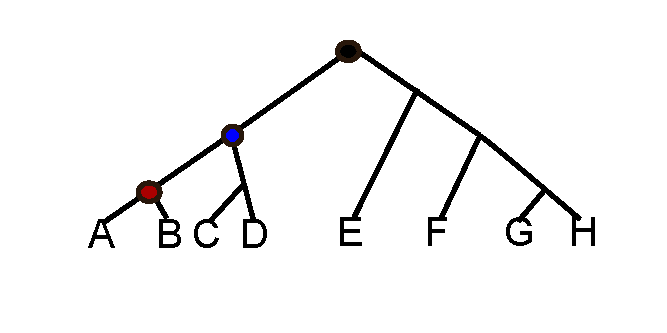
\includegraphics[width=0.60\linewidth]{{background/phylogeny}.pdf}\\
  \caption[]{A rooted phylogenetic tree.}
\end{subfigure}
\begin{subfigure}[htpb]{\textwidth}
  \centering
  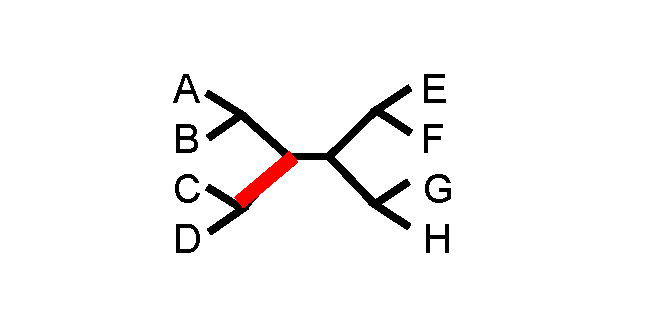
\includegraphics[width=0.60\linewidth]{{background/unrooted_phylogeny}.pdf}\\
  \caption[]{An unrooted phylogenetic tree.}
\end{subfigure}
\caption[Example of rooted and unrooted trees.]{\label{back:phylo_tree} Example of a) a rooted phylogenetic tree, and b) the unrooted version of the same tree.  In the rooted tree, the red node is the MRCA of species $A$ and $B$, and the blue node is the MRCA of $A$ and $C$.  The black node is the MRCA of all species in the tree.  In the unrooted tree, the red edge represents the bipartition $\{CD|ABEFGH\}$.}
\end{figure}

\paragraph{Multiple Sequence Alignment.}
Biomolecular sequences are represented as a character string over an $n$-letter alphabet.  The most common alphabets are the 4-letter alphabets for nucleotides ($\{A,T,C,G\}$ for DNA and $\{A,U,C,G\}$ for RNA) and the 20-letter alphabet for amino acid sequences.  Because DNA is inherited from parent to child, the biomolecular sequences can be used to reconstruct the evolutionary history of present day organisms. %However, the ancestral organisms that gave rise to the current species are lost, thus, the evolutionary history of present day sequences must be inferred from sequences collected in the present; 
%; sequences from ancestral populations are .  
\textbf{Should add some extra background on uses of MSA, functional annotation of proteins/environmental reads, detecting conserved domains in proteins, sequence database search, remote homology detection, phylogeny estimation, etc... so that way can motivate why MSA is important}

A fundamental process for understanding the relationship between the different sequences is to estimate an alignment on the sequences.  A \emph{Multiple Sequence Alignment} (MSA) is a data structure that represents the evolutionary relationships between the individual characters of a set of sequences.  An MSA on a set of sequences is defined by an $n x m$ matrix in which each row is a sequence interspersed with gap characters (``-'').  Gap characters represent historical insertion and deletion events (called ``indel'' events).  Each column in the matrix represents a site of common evolutionary origin.  If a pair of characters descended from the same ancestral character, then they are called \emph{homologous} and will be in the same column in the MSA  Homology is a transitive property, so if a nucleotide $A$ is homologous to nucleotide $B$ and $C$, then nucleotides $B$ and $C$ are also homologous to each other.  Figure~\ref{back:alignment} shows an example of a MSA.  The goal of an MSA is infer sites of shared homologies between the different sequences.

\end{figure}[htpb]{\textwidth}
\centering
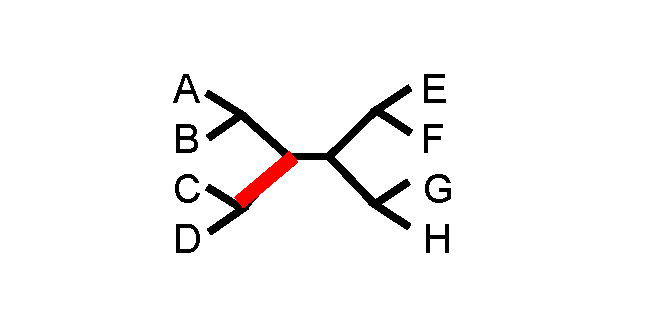
\includegraphics[width=0.60\linewidth]{{background/unrooted_phylogeny}.pdf}\\
\caption[Example of a MSA.]{\label{back:alignment} Example of a MSA on S1 to Sn.  Originally, the sequences are unaligned and of different lengths.  The sequences are aligned by inserting gaps into the sequences such that homologous characters line up in the same site.}
\end{figure}

\paragraph{Simulation study.}
There are many different methods for estimating an MSA and for estimating a phylogenetic tree.  Because it's impossible to know the true history for a set of sequences, simulation studies are performed to test the performance of the different methods.

A typical molecular simulation study begins by generating a rooted model tree that represents the true evolutionary history of the set of sequences.  The model tree can be generated by using a phylogenetic tree generated from a previous study, or it can be generated by using a stochastic model of speciation (see ~\cite{Aldous2001} for review of tree models).  Once a model tree has been generated, a stochastic model of sequence evolution is selected~\cite{todo}, as well as a model of indel events~\cite{todo}.  These models include the rate of substitutions, as well as the rate of insertion and deletion events, and the size of the indels events, in terms of the number of characters inserted/deleted.  Once all the parameters have been selected, a random sequence is generated at the root, and it is simulated down the model tree with substitution and indel events (see Fig.~\ref{back:seq_evo}).  The true sequence is known at each internal node, as well as the history of the mutation patterns.  Thus, at the very end of the simulation, the true MSA and true phylogeny of the sequences are known and can be used to compare the accuracy of MSA and phylogeny estimation methods. 

\end{figure}[htpb]{\textwidth}
\centering
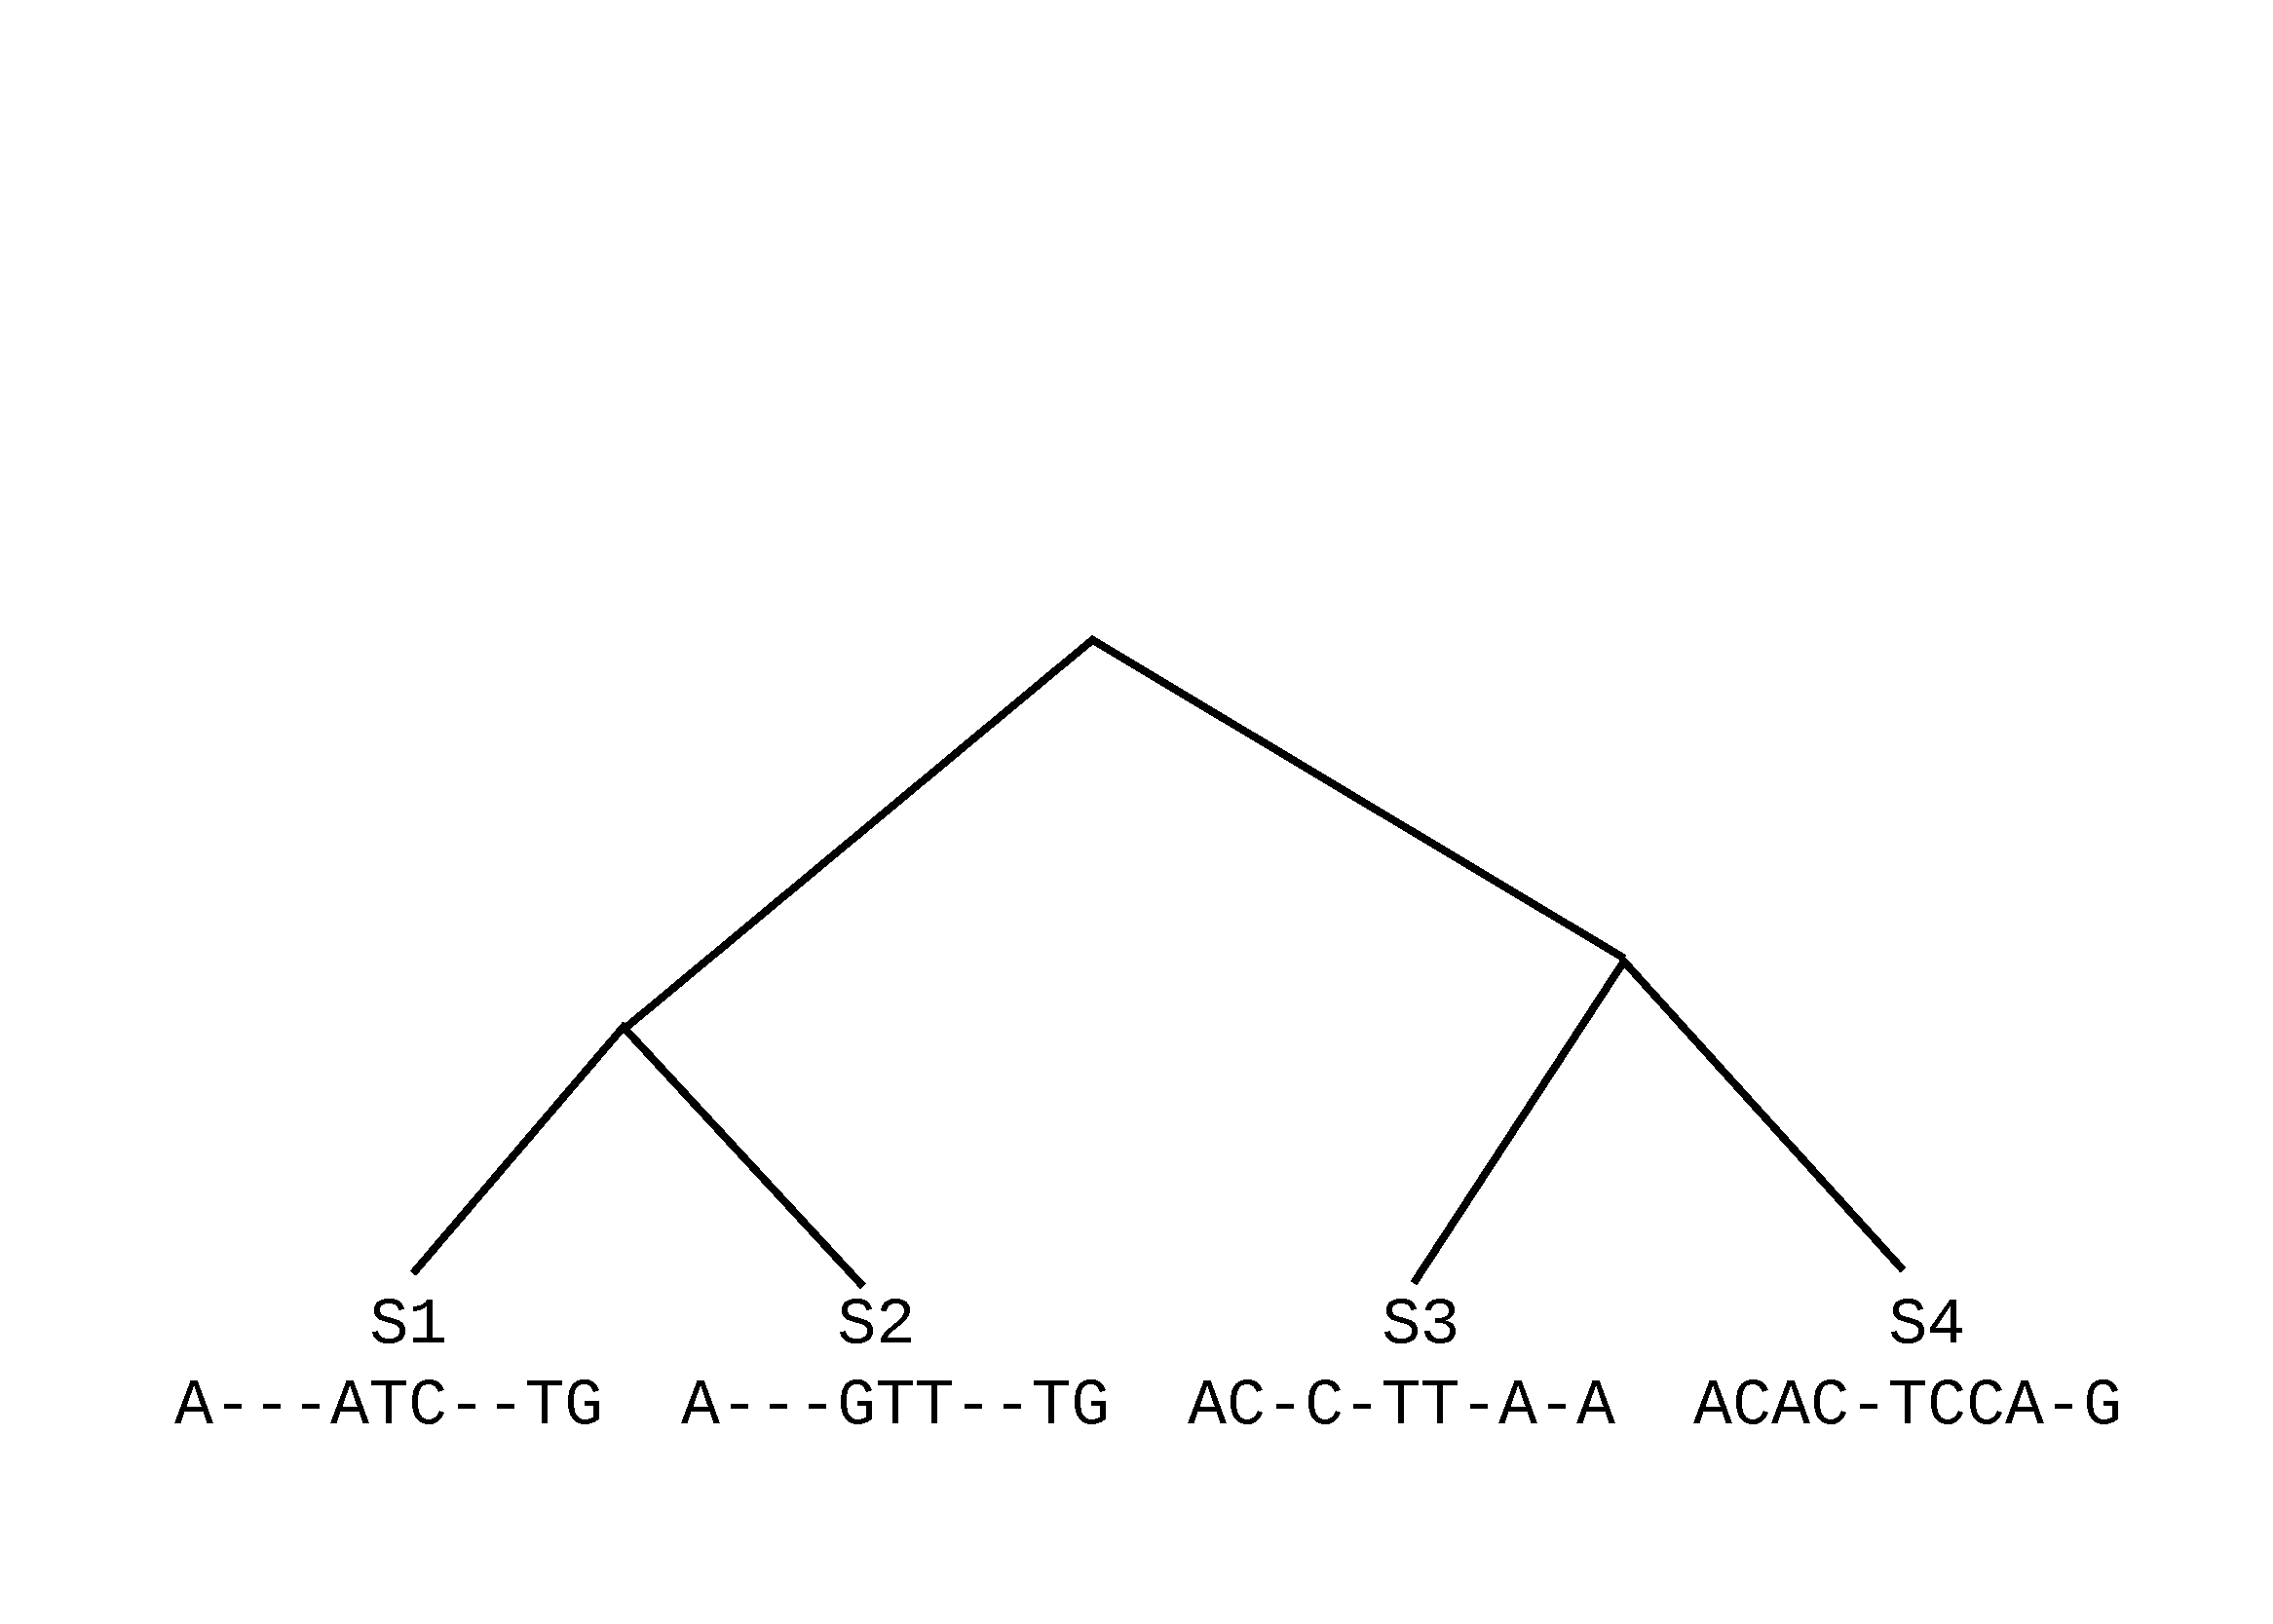
\includegraphics[width=0.60\linewidth]{{background/seq_evolution}.pdf}\\
\caption[Example of sequence evolution.]{\label{back:seq_evo} Example of sequence evolution down a model tree.  The original sequence at the root is ``ATCG''.  Through a series of insertions (colored blue), deletions (colored red), and substitutions (colored green), the root sequence evolves to 4 new sequences. The goal of a molecular phylogenetic study is to infer from the unaligned sequences the true alignment and phylogeny.}
\end{figure}

% \emph{Phylogenetics} is the study of the evolutionary relationship between different organisms, and phylogenies are a product of a phylogenetic study.  A typical molecular phylogenetic study begins by collecting biomolecular sequences (DNA, RNA, or amino acid sequences) from the species of interest.  The sequences come from a homologous


% One common representation of a phylogeny is through a phylogenetic tree.  Figure~\ref{back:phylo_tree} shows an example of a rooted phylogenetic tree.  
% The leaves of the tree represent the organisms of interest.  Throughout my dissertation, I will refer to the leaves of the tree as species, taxa, or sequence, interchangeably.  The relationship between the different species can be inferred from the tree.  For example, species $A$ and $B$ are more closely related than $A$ and $C$ because $A$ and $B$ share a more recent common ancestor (red node) than $A$ and $C$ (blue node).  Each internal node represents a \emph{speciation event}, in which a lineage splits into two new lineages.  The root of the phylogeny represents the most recent common ancestor of all the species.  

% The theory of universal common ancestry states that all living organisms have shared evolutionary history, or in other words, all extant species descended from a common ancestor.  Thus, as DNA is passed on from parent to child, DNA and biomolecular sequences that are derived from DNA (RNA and amino acids), are often collected and used to infer phylogenies.  

% \textbf{NAM:Add more formal definition, citations; include uses of phylogenies in virology, medicine production, etc..., show unrooted trees, also, discuss models of sequence evolution, indels mutation?}.

\section{MSA estimation}\label{back:alignment}
Computing an MSA is typically formulated as an optimization problem of minimizing the dissimilarity between different sequences across the sites in the alignment.  One simple dissimilarity metric used is the sum-of-pairs (SP) score~\cite{todo}.  The SP score is computed by summing the total number of mismatches (pair of aligned ``non-gap'' characters that do not match) and indels (any ``non-gap'' character aligned to a ``gap'' character) over all pairs of sequences in the MSA.  Figure~\ref{back:sp_score}a shows the computation of the SP score for a pair of sequences.  Figure~\ref{back:sp_score}b shows the SP score for two MSAs on the same set sequences.  In this example, the bottom MSA has a lower SP score and would be considered more accurate under the SP score optimization criterion.  

\end{figure}[htpb]{\textwidth}
\begin{figure}[htpb]
\begin{subfigure}[htpb]{\textwidth}
  \centering
  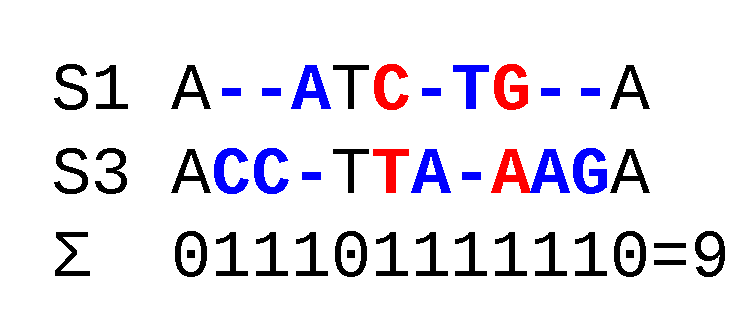
\includegraphics[width=0.60\linewidth]{{background/sp_scoring}.pdf}\\
  \caption[]{Computing SP score for 2 sequences.}
\end{subfigure}
\begin{subfigure}[htpb]{\textwidth}
  \centering
  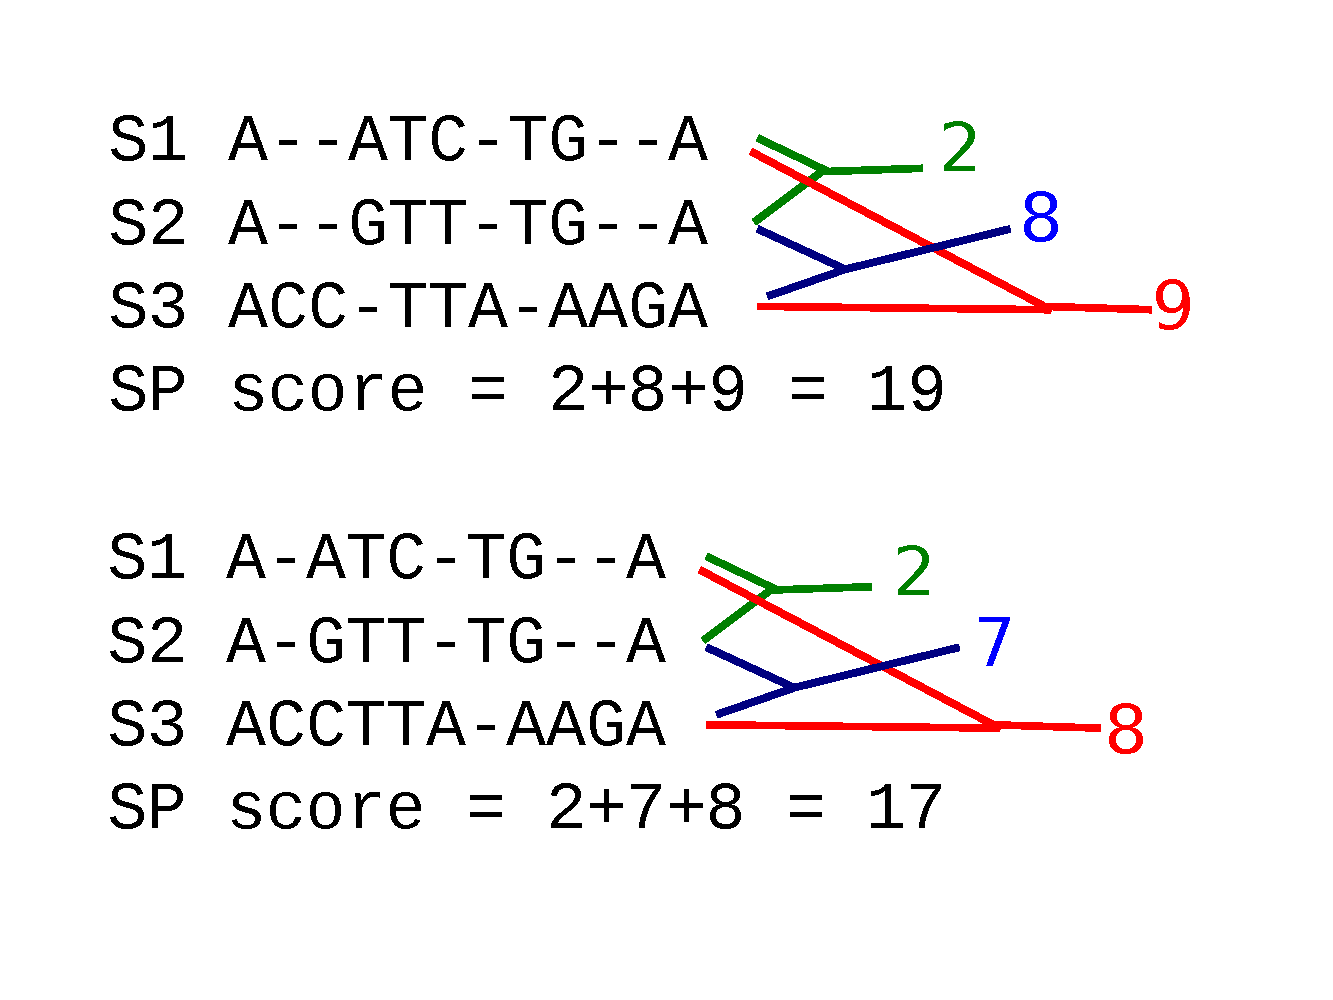
\includegraphics[width=0.60\linewidth]{{background/sp_score}.pdf}\\
  \caption[]{Computing SP score for an MSA.}
\end{subfigure}
\caption[Example of scoring MSAs.]{\label{back:sp_score} Example of a) computing the SP score for a pair of sequences, and b) the SP scores for two different MSAs of the same set of sequences.  In a), mismatches are highlighted red, and indels are highlighted blue.  The SP score is the sum of the total number of mismatches and indels.  In b) the SP scores for each pair of sequences are shown.  The total SP score for an MSA is the sum of all the pairwise SP scores.  In this example, the lower MSA has lower SP score and is more desirable under the SP score optimization criterion.}
\end{figure}

Computing an MSA that optimizes SP score (and many other similar distance metrics) is NP-complete~\cite{Wang1994,Bonizzoni2001} and thus, finding an exact solution is computationally intractable for large datasets.  Heuristics have been developed for MSA estimation(see~\cite{Notredame2002,Thompson2011} for survey and comparison of current methods), including progressive methods which build an MSA by progressively aligning pairs of sequences and then merging the alignments using tree~\cite{todo}, and iterative methods which combine progressive methods and iteration so that the estimated MSA is reused to estimate a better MSA~\cite{todo}.  However, these methods suffer in that they do not scale linearly with the number of sequences to be aligned~\cite{Notredame2002}.

Another class of MSA estimation methods include methods that use profile Hidden Markov Models (HMM).  A profile HMM is a statistical representation of an MSA (see Section~\ref{back:hmm} for more indepth overview).  HMM methods take an existing MSA and computes a profile HMM from that MSA.  Sequences are then independently aligned to the profile.  Thus, profile HMM methods scale linearly with the number of sequences to align to an existing MSA.  However, the quality of the HMM is heavily impacted by the quality of the existing MSA, and on datasets containing evolutionary divergent sequences, the ability for HMM methods to accurately detect homologies degrades~\cite{Moriyama2006,Finn2010}.

\paragraph{Comparing alignments.}  If a true alignment is known via simulation study, or a high quality curated alignment has been estimated, one can compare the quality of an estimated alignment by examining the percentage of shared and missing homologies with respect to the reference alignment.  One pair of metrics that can be used to score the quality of an estimated MSA are the sum-of-pairs false negative (SPFN) and the sum-of-pairs false positive (SPFP) rates~\cite{todo}.  The SPFN rate is defined as the total of homologies in the true alignment that are not found in the estimated alignment, normalized by the total homologies in the true alignment.  Similarly, the SPFP rate is defined as the total of homologies in the estimated alignment that are not found in the true alignment, normalized by the total homologies in the estimated alignment.  

In my dissertation, I report both metrics, as well as the average of the two rates.  In addition, I also report the total column (TC) error rate on protein datasets.  This the number of columns in the true alignment that are exactly recovered in the estimated alignment, normalized by the total columns in the true alignment.  This metric is of interest when the goal is to examine how well alignment methods recover conserved domains in the alignment.

%As one might expect, estimating every single homology correctly at a site when there are many sequences is difficult for all but the most conserved sites.  

%\textbf{Build figure showing how SPFN and SPFP is computed}

\section{Phylogeny estimation}\label{back:tree_estimation}
Many different methods exist for estimating a phylogenetic tree from an MSA.  


\paragraph{Comparing trees.}  

Trees can be compared by examining the edges that they share in common and the edges that are unique to each tree.  Each edge in the tree defines a bipartition.  For example, in Figure \ref{back:phylo_tree}(b), the red edge represents the bipartition $\{CD|ABEFGH\}$ (note that $\{CD|ABEFGH\}$ is identical to $\{ABEFGH|CD\}$).  Removal of this edge separates $CD$ from $ABEFGH$.  A tree can be uniquely identified by its set of bipartitions.  Thus, Figure \ref{back:phylo_tree}(b) can be uniquely identified by the bipartition set $\{\{AB|CDEFGH\}, \{CD|ABEFGH\}, \{EF|ABCDGH\},\{GH|ABCDEF\},$ $\{ABCD|EFGH\}\}$ (trival bipartitions that split a leaf node from the remaining leaves of the tree does not need to be listed as these bipartitions will be found in all trees that share the same leaf set).

\textbf{Nam:  Discuss that these trees presented are binary trees, and that they can also contain polytomies.}

One metric that can be used to compare tree topologies is by looking at the total number of bipartitions that are unique to each tree.  This metric is known as the Robinson–Foulds (RF) distance~\cite{RF}.  More formally, let $S_1$ be the set of bipartitions in $T_1$ and $S_2$ be the set of bipartitions in $T_2$, then the RF distance is defined as: $RF=|S_1\cup S_2|-|S_1\cap S_2|$. Typically, this metric is normalized by the total number of bipartitions in $T_1$ and $T_2$.  

If the true tree is known, then the error of an estimated tree can be measured by the percentage of bipartitions in the true tree that are not recovered in the estimated tree (the false negative rate), and by the percentage of bipartitions in the estimated tree that are not in found in the true tree (the false positive rate), and the average of these two rates (Robinson–Foulds rate).  More formally, if $T_1$ is the true tree and $T_2$ is the estimated tree, then the false negative (FN) rate is defined as: $FN=1-\frac{|S_1\cap S_2|}{|S_1|}$.  Similarly, the false positive (FP) rate is defined as: $FP=1-\frac{|S_1\cap S_2|}{|S_2|}$.  For binary trees, $FN=FP=RF$.  The FN rate is also known as the missing branch rate as it is the percentage of branches that are missing from the estimated tree, and I will interchangeably use these two terminologies.  

My dissertation primarily reports the missing branch rate as the error metric for comparing trees.  For simulated datasets, the model trees are binary trees, thus reporting missing branch rate is identical to reporting the FP and RF rates.  For biological datasets, the reference trees are ML trees estimated on a curated alignment, with only highly support edges retained.  Thus, the reference trees on biological datasets are non-binary, and the FP and FN rates will differ.  It is extremely easy for a method to estimate a tree with low FP rate by random chance; the method could estimate a highly unresolved tree.  It is exponentially more difficult for a method to estimate a tree with low FN rate by random chance.  Thus, reporting the FN rate for biological datasets is an appropriate measure. 

Figure~\ref{back:tree_error} shows an example of a true tree and an estimated tree.  Each tree contains 5 bipartitions.  The bipartitions $\{AB|CDEFGH\}$ and $\{CD|ABEFGH\}$ are found in the true tree, but not present in the estimated tree.  Thus, missing branch rate 20\%.  Similarly, the bipartitions $\{AC|BDEFGH\}$ and $\{BD|ACEFGH\}$ are found in the estimated tree, but not present in the true tree, yielding an FP rate of 20\%.

\textbf{Nam:  Add a little about non-binary trees, and that this dissertation focuses on FN rates because for simulation results FN=FP.  However, for biological datasets, we have bootstrap reference trees that are non-binary and so we focus on how well we can recover highly supported edges.  }


\begin{figure}[htbp]
\centering
{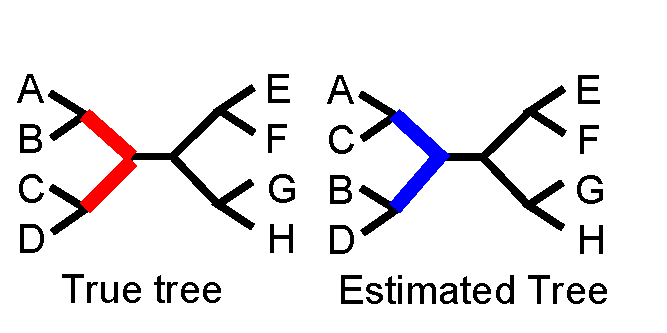
\includegraphics[width=0.60\textwidth]{background/unrooted_phylogeny_a}}
\caption[Computing error metrics of estimated tree.]{An example of the true tree and the estimated tree.  The estimated tree has an FN of $\frac{2}{5}$ (two bipartitions colored red in the true tree are not found in the estimated tree; five bipartitions in true tree) and has an FP of $\frac{2}{5}$ (two bipartitions colored blue in the estimated tree are not found in the true tree; five bipartitions in estimated tree).}  
\label{back:tree_error}
\end{figure}



%Each edge in the tree defines a bipartition.  For example, in Figure \ref{back:phylo_tree}(b), the red edge represents the bipartition $\{CD|ABEFGH\}$ (note that $\{CD|ABEFGH\}$ is identical to $\{ABEFGH|CD\}$).  Removal of this edge separates $CD$ from $ABEFGH$.  A tree can be uniquely identified by its set of bipartitions.  Thus, Figure \ref{back:phylo_tree}(b) can be uniquely identified by the bipartition set $\{\{AB|CDEFGH\}, \{CD|ABEFGH\}, \{EF|ABCDGH\},\{GH|ABCDEF\},$ $\{ABCD|EFGH\}\}$ (trival bipartitions that split a leaf node from the remaining leaves of the tree does not need to be listed as these bipartitions will be found in all trees that share the same leaf set).

%\textbf{Nam:  Discuss that these trees presented are binary trees, and that they can also contain polytomies.}



%When working with empirical datasets, however, the true evolutionary history of the sequences is unknown.   Thus, we can only give a best estimate of the true tree by using the most accurate phylogeny estimation technique on reference trees are estimated on curated alignments.  

% Start with a simplified view of sequence evolution.  There is a DNA sequence at the root.  It evolves down tree through series of substitutions and indels (Fig.~\ref{back:mutations}).  At the end of the process is are sequences that are homologous; they all descended from a common sequence.  A phylogenetic analyses will typically begin by collecting a set of homologous sequences from a common source, such as gene protein sequence.  This is the end result of the sequence evolution process; the history of the changes is lost.  Due to insertion and deletion events, the sequences are all of different length.  Typically a first step in estimating a phylogeny is to first estimate a \emph{Multiple Sequence Alignment} (MSA).  An MSA is a matrix where each row contains a sequence and each column represents shared homology for all biomolecular characters in that column.  

% There are many different methods for estimating MSA, including Bayesian techniques (BAli-Phy) that co-estimate alignments and trees, progressive alignment techniques that use a guide tree to pairwise align the sequences (ClustalW, T-COFFEE), iterative methods that use a guide tree, but iterate to obtain better guide trees (Muscle, Mafft, SATe).  

\section{Hidden Markov Models}\label{back:hmm}

\textbf{Add text discussing how to use profile HMM to align a sequence; add the figure of the profile HMM, discuss model (match state, insertion state, deletion state, states represent sites, discuss that it's a probabilistic model of an MSA, discuss how a sequence is aligned through dynamic programming}
% \begin{figure}[htbp]
% \centering
% {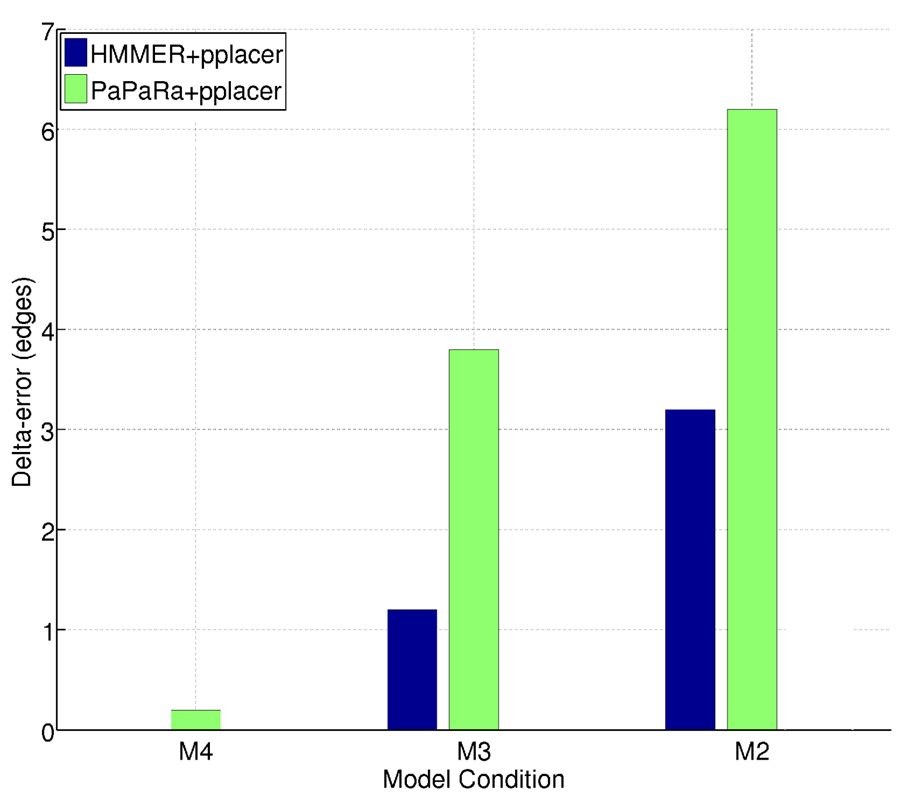
\includegraphics[width=0.80\textwidth]{sepp/hmmer_papara}}
% \caption[Comparison of HMMALIGN+pplacer and PaPaRa+pplacer.]{Comparison of HMMALIGN+pplacer and PaPaRa+pplacer under 3 different model conditions, ranked in order of increasing rate of evolution.  Thus, M4 is the slowest evolving dataset, and M2 is the fastest evolving dataset.  The number of sequences in the backbone set is 500 for all model conditions.} 
% \label{background:initial}
% \end{figure}
\section{Applications of profile HMMs}\label{back:app}
\subsection{Phylogenetic placement}
As I briefly mentioned in Chapter~\ref{intro}, phylogenetic placement is a method for inserting query sequences into an existing phylogenetic tree.  This problem arises in the analyses of short DNA fragments taken from an environmental sample~\cite{todo}.

I now formally describe the phylogenetic placement problem as follows:

%\textbf{Add text before the formal description on why phylogenetic placement is necessary.  Good for analyzing short fragmentary reads because most traditional alignment methods assume global alignment, need local alignment for shorter fragments.  In addition, under the context of AToL, can build a large tree by aligning to only a backbone alignment instead of all sequences against all other sequences, and then inserting into an existing tree instead of estimating an entire tree on all sequences.  Thus phylogenetic placement may be a method for getting at a tree of all life.}
%This method is useful in the analyses of short fragmentary reads.  When a dataset consists of sequences of heterogeneous lengths containing both full-length and fragmentary sequences, attempting to globally align the sequences together may result in very gappy alignments of the fragmentary reads.  A better approach is to estimate an alignment and tree on the full-length sequences, and then insert the remaining fragmentary sequences into tree.  The advantage

%Many traditional alignment techniques perform global alignment and assume all the sequences are full-length and of roughly equal size.  When this assumption is violated, such as in the case of aligning fragmentary reads, global alignment methods may end up inserting many gaps to get the fragmentary sequence to align well to the full-length sequences~\cite{todo}.  

\noindent{\em Phylogenetic Placement Problem. }
\begin{itemize}
\item Input: the {\em backbone} tree $T$ and {\em backbone} alignment $A$ on set $S$ of full-length sequences,
and query sequence $s$.
\item Output: tree $T'$ containing $s$ obtained by adding $s$ as a leaf to
$T$.
\end{itemize}

The query sequences

Several methods have been developed for this problem using
the following two steps:
\begin{itemize}
\item Step 1: insert $s$ into alignment $A$ to produce the
{\em extended alignment} $A'$
\item Step 2: add $s$ into $T$ using $A'$, optimizing some criterion
\end{itemize}
Methods for the first step 
include HMMALIGN~\cite{Eddy1998}
and the recently introduced PaPaRa~\cite{Berger2011a} method.  
Methods for the second step include 
 EPA~\cite{Berger2011} and pplacer~\cite{Matsen2010}, which
seek to optimize maximum likelihood
(pplacer also provides a Bayesian approach).
Methods for phylogenetic placement can therefore
be described
by how they handle each step.
Three such methods
include PaPaRa+EPA~\cite{Berger2011a},
HMMALIGN+EPA~\cite{Berger2011},
and HMMALIGN+pplacer~\cite{Matsen2010}.
EPA and pplacer are comparably 
fast and have almost identical 
placement accuracy,
  but have somewhat
different memory usage and algorithmic features~\cite{Matsen2010};
hence the differences between HMMALIGN+EPA and HMMALIGN+pplacer
do not impact the placement accuracy, and have a minor
impact on running time and memory usage.
The two techniques for computing the extended alignment,
PaPaRa and HMMALIGN, are very different.
HMMALIGN computes a HMM to represent the full-length alignment,
and then aligns each query sequence to that HMM.  In contrast,
PaPaRa uses RAxML to estimate ancestral state 
vectors for each branch in the
tree, aligns the query sequence to every ancestral state
vector, selects the alignment that had the best score and uses
it to extend
alignment $A$ to include $s$.
Consequently, PaPaRa is computationally more 
expensive than HMMALIGN~\cite{Berger2011a}, but EPA placements
of query sequences based upon PaPaRa extended alignments can be
more accurate than EPA placements based upon HMMALIGN extended alignments.
However, the improvement in topological accuracy reported~\cite{Berger2011a}  for
PaPaRa+EPA over HMMALIGN+EPA was
relatively small, with PaPaRa+EPA placing
query sequences on average
about one edge closer to the correct
location, out of 799 edges. 
Therefore, PaPaRa+EPA and HMMALIGN+EPA are very close
in terms of placement accuracy, although substantially different
in terms of running time.  

\paragraph{Comparing placement accuracy.}  
The metric used in my dissertation for measuring the accuracy of placement is the change in missing branch rate of the backbone tree before and after insertion of the query sequence (called \deltafn ).  More formally, if $FN$ is the number of missing branches in the backbone tree $T$, and $FN'$ is the number of missing branches in $T'$, then \deltafn$=FN'-FN$.  Figure~\ref{back:placement_error} shows an example of this computation.  Let the initial backbone tree have 0 FN.  After the insertion of the query sequence $s$ into $T$, $T'$ is missing bipartitions $\{As|BCDEFGH\}$ and $\{ABs|CDEFGH\}$ (bipartitions colored red in Fig.~\ref{back:placement_error}).  The resulting \deltafn~is 2.

\textbf{Nam: discuss possible case of \deltafn~ being negative.}

\begin{figure}[htbp]
\centering
{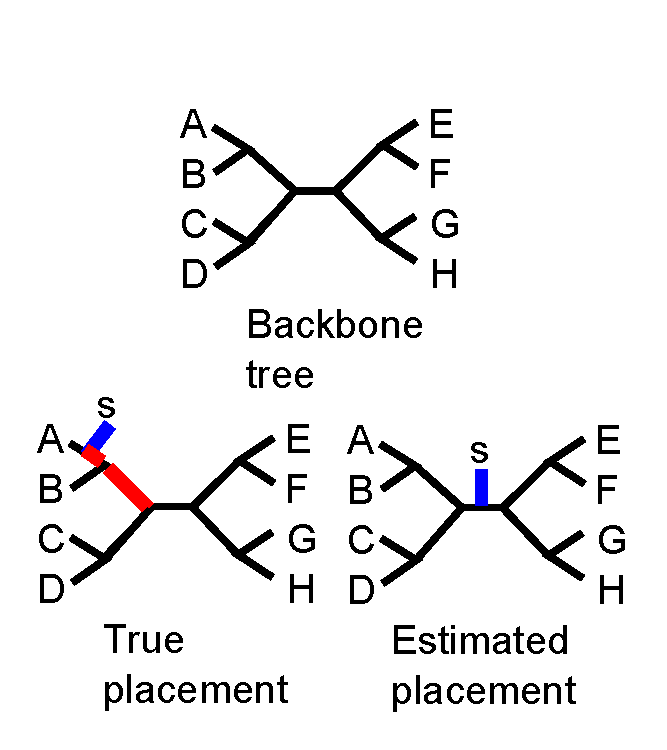
\includegraphics[width=0.60\textwidth]{background/unrooted_phylogeny_b}}
\caption[Computing \deltafn~error of query sequence placement.]{\label{back:placement_error}An example computing the \deltafn~error of query sequence placement.  The backbone tree originally has 0 missing branches.  After insertion of the query sequence $s$, the estimated tree $T'$ is missing 2 bipartitions that are found in the true true (missing edges colored red).  Thus, the \deltafn~is 2.}
\end{figure}

% For the most likely placement\footnote{Multiple possible placements for
% each read, along with the likelihood of each placement,
% are also provided by pplacer.} of each fragmentary
% read, I first calculate the number of missing branches compared to the 
% reference tree. 
% This number in isolation is hard to interpret, for at least two reasons.
% In the case where \sate~alignment/tree is the input, the backbone tree itself
% contains error. The error of the initial backbone tree is a lower bound on the
% tree error after placement of reads (in fact it is a rather liberal lower bound,
% as the optimal placement of fragments can still have errors higher than the
% initial tree).
% In the case where true or curated alignment/tree is 
% the input, the initial tree has no
% error, but I can still establish useful lower bounds of the tree error. 
% This can be done by using the reference alignment of query sequences 
% to be the backbone alignment as input to the \pplacer. 
% The resulting placement of query sequences
% is the best one can realistically hope for.

% To account for the lower bounds described above,
% I also define and report 
% the ``delta error" for each technique,  as follows.
% For each read $s$ placed on the \sate~backbone tree, 
% I report the difference between
% the number of missing branches of the initial 
% backbone tree 
% and the number of missing branches after placement of $s$.
% When the backbone tree is 
% the reference (true or curated) tree, 
% I report the
% difference between the number of missing branches of the tree produced by
% placement of $s$ according to the 
% reference alignment of $s$ to $S$ and 
% the number of missing branches
% of the tree after placement of $s$.
% In all cases, 
% the number of missing branches in each tree is defined with
% respect to the reference tree for the taxa in the given tree.
% Thus, the number of missing branches in the backbone trees is
% defined by the reference tree on the set $S$ of backbone taxa, and the
% number of missing branches in the tree produced by placing the
% query sequence into the backbone tree is defined by the
% reference tree on the set $S \cup \{s\}$.


% Note that in the case where the backbone tree is the reference tree, 
% the number of missing branches is
% equal to the node distance between the correct placement of reads and
% actual placements, the error used in the literature\cite{Berger2011,Matsen2010,Berger2011a}. 
% However, this edge distance is not as meaningful as the 
% number of missing branches with respect to either the true or
% curated tree, since estimated trees will generally have error.

\subsection{Metagenomic analyses}\label{back:metagenomic}
Traditionally, bacterial species of interest from an environmental sample were identified by first culturing a clonal colony of the species in a laboratory environment, and then sequencing the genetic material directly from the colony using Next Generation Sequencing (NGS) technology.  The output of NGS technology is millions of short DNA fragments called reads.  As all the reads come from the same species, the fragments can be assembled together into longer sequences called contigs, and from the contigs, the genome of the original species could be estimated and the species could be taxonomically classified.

However, an estimated 99\% of all microbial life cannot be cultured in lab~\cite{todo}, and thus the genomes of these organisms cannot be sequenced using traditional methods.  Metagenomic analyses provide a window into the organisms present in an environmental sample by sequencing the genetic material directly from the sample.  This process poses a new problem, though, as now the reads come from all the species present in the sample, making assembly extremely difficult~\cite{todo}.  One of the fundamental challenges in a metagenomic study is the taxonomic classification of the metagenomic reads.  

Providing taxonomic labels to metagenomic sequences requires
extrapolating the knowledge contained in sequence databases to
previously unseen DNA strings.  Simple similarity-based approaches
(e.g., picking the best database hit as the best `guess' at the
taxonomic label) have been shown to be insufficiently
accurate \cite{closest-blast-hit}, leading to the development of 
new and more sophisticated methods.

Recently developed methods improving
on the simple similarity-based approaches include 
(a) composition-based approaches that rely on
various machine learning techniques 
(Support Vector Machines in
PhyloPythia and PhyloPythiaS \cite{McHardy2007a, Patil2011}, 
Interpolated Markov Models in Phymm 
\cite{Brady2011},
Bayesian models in NBC \cite{Rosen2011}, or neural networks~\cite{SOM2006}) to
classify sequences based on their DNA composition (usually based on
the frequency of short k-mers),
(b)  more sophisticated analyses of
similarity search results (e.g., using least-common-ancestor
aggregation in Megan \cite{Huson2007}, or classifiers built from similarity
search results as done in MetaPhyler \cite{Liu2011d,Liu2011}, 
MetaPhlAn \cite{Segata2012a}, and mOTU \cite{Sunagawa2013}
or protein profiles in Carma \cite{Gerlach2011b}), and
(c) combinations of
multiple approaches (e.g., composition and similarity based approaches
in PhymmBL \cite{Brady2009}).  
Some of these approaches (e.g., most of the
composition-based approaches) can be applied to any DNA sequence,
while others are specific to a reference collection of carefully
selected genes (e.g., MetaPhyler, MetaPhlAn, and mOTU use a collection of
universal or clade-specific marker genes).  These
``marker-gene" methods can
achieve much higher recall than other
approaches~\cite{Liu2011d} for sequences from the marker genes, but 
can only classify a small
fraction of all sequences (namely, those that match the 
selected marker genes). 

Abundance profiling, also called ``phylogenetic profiling", 
seeks to estimate the relative
abundance of the species (or
genera, or families, etc.) within a sequence dataset.
While many methods produce these estimates by characterizing
most (or all) of the sequences in the dataset, marker-based methods
produce these estimates by characterizing only those
sequences that match the marker genes they rely on.
Since the marker genes are supposed to be single
copy and universal, these estimations do not need to
be corrected for the copy number in each genome, or for
missing data. 
However, the restriction to sequences that match the marker genes
has the potential to reduce accuracy since it means only a subset
of the sequences are characterized.

\paragraph{Taxonomic identification}\label{back:taxonomic_id}
\textbf{NAM:Add more formal definition, citations}.
\paragraph{Taxonomic profiling}\label{back:taxonomic_profiling}
\textbf{NAM:Add more formal definition, citations}


% Metagenomic studies of microbial communities commonly generate
% millions to hundreds of millions of sequencing reads.  The assignment
% of accurate taxonomic labels to these sequences is a critical
% component in many analyses, but is
% complicated by the fact that the majority of the organisms
% found in environmental or host-associated communities cannot be easily
% cultured in a laboratory, and an even smaller number have been
% sequenced, even partially.  Thus, these commonly encountered organisms
% are largely absent from existing databases of known genomes and genes.
% Providing taxonomic labels to metagenomic sequences requires
% extrapolating the knowledge contained in sequence databases to
% previously unseen DNA strings.  Simple similarity-based approaches
% (e.g., picking the best database hit as the best `guess' at the
% taxonomic label) have been shown to be insufficiently
% accurate \cite{closest-blast-hit}, leading to the development of 
% new and more sophisticated methods.
% 
% Recently developed methods improving
% on the simple similarity-based approaches include 
% (a) composition-based approaches that rely on
% various machine learning techniques 
% (Support Vector Machines in
% PhyloPythia and PhyloPythiaS \cite{McHardy2007a, Patil2011}, 
% Interpolated Markov Models in Phymm 
% \cite{Brady2011},
% Bayesian models in NBC \cite{Rosen2011}, or neural networks~\cite{SOM2006}) to
% classify sequences based on their DNA composition (usually based on
% the frequency of short k-mers),
% (b)  more sophisticated analyses of
% similarity search results (e.g., using least-common-ancestor
% aggregation in Megan \cite{Huson2007}, or classifiers built from similarity
% search results as done in MetaPhyler \cite{Liu2011d,Liu2011}, 
% MetaPhlAn \cite{Segata2012a}, and mOTU \cite{Sunagawa2013}
% or protein profiles in Carma \cite{Gerlach2011b}), and
% (c) combinations of
% multiple approaches (e.g., composition and similarity based approaches
% in PhymmBL \cite{Brady2009}).  
% Some of these approaches (e.g., most of the
% composition-based approaches) can be applied to any DNA sequence,
% while others are specific to a reference collection of carefully
% selected genes (e.g., MetaPhyler, MetaPhlAn, and mOTU use a collection of
% universal or clade-specific marker genes).  These
% ``marker-gene" methods can
% achieve much higher recall than other
% approaches~\cite{Liu2011d} for sequences from the marker genes, but 
% can only classify a small
% fraction of all sequences (namely, those that match the 
% selected marker genes). 
% 
% Abundance profiling, also called ``phylogenetic profiling", 
% seeks to estimate the relative
% abundance of the species (or
% genera, or families, etc.) within a sequence dataset.
% While many methods produce these estimates by characterizing
% most (or all) of the sequences in the dataset, marker-based methods
% produce these estimates by characterizing only those
% sequences that match the marker genes they rely on.
% Since the marker genes are supposed to be single
% copy and universal, these estimations do not need to
% be corrected for the copy number in each genome, or for
% missing data. 
% However, the restriction to sequences that match the marker genes
% has the potential to reduce accuracy since it means only a subset
% of the sequences are characterized.

% \paragraph{Taxonomic identification through phylogenetic placement.}
% One approach toward taxonomic identification is through phylogenetic placement.  The evolutionary relationship between the the query sequence and the backbone sequences can be inferred from the placement location.  For example, in Figure~\ref{tipp:placement}, $Q1$ is placed closest to Species $A1$, and thus, it can be inferred that $Q1$ is more closely related to Species $A1$.  Similarly, $Q2$ is more closely related to Species $A1$ and $A2$ than to Species $B1$ and $B2$.  Thus, one simple technique for identifying a query sequence is to classify it by the LCA of its sibling leaf nodes.  Thus, $Q1$ would be classified as Species $A1$ (its only sibling leaf node is Species $A1$) and $Q2$ would be classified as Genus $A$ (its sibling leaf nodes are Species $A1$ and Species $A2$).  
% 
% \begin{figure}[htpb]
% \begin{center}
% {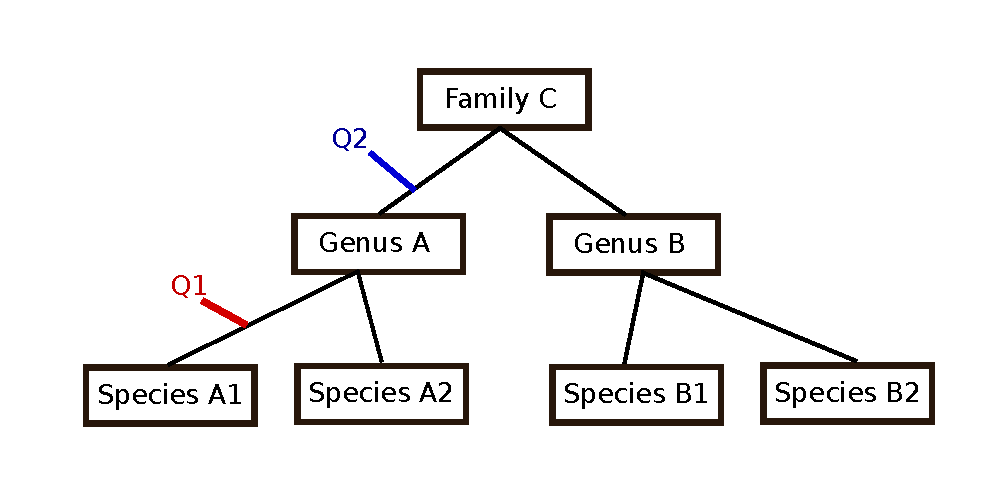
\includegraphics[scale=0.8]{tipp/placement.pdf}}
% \end{center}
% \caption[Taxonomic classification using phylogenetic placement]{\label{tipp:placement} Taxonomic classification using phylogenetic placement.  The leaf nodes of the rooted backbone tree are labeled with the species name.  Each query sequences is placed onto an edge in the backbone tree and is classified by the LCA its sibling leaf nodes.}
% \end{figure}
% 
% Using this approach, I compared SEPP and HMMALIGN+pplacer for taxonomic identification under a \emph{leave-species-out} experiment.  Under a leave-species-out experiment, the species of the query sequence is removed from the backbone alignment and tree, simulating the classification of a novel species.  Thus, while the species of the query sequence cannot be correctly identified, the remaining taxonomic lineage (genus, family, etc...) can still be correctly classified.  The fragments were simulated under differring models and rates of sequencing error.  
% 
% Figure~\ref{tipp:preliminary_sepp} shows that SEPP is more sensitive than HMMALIGN+pplacer under the hardest model condition (``454\_3''), classifying more fragments correctly, especially at the phylum level.  Both methods tend to classify the large majority of the fragments, leaving very few fragments unclassified.  This results in a very high false positive rate, especially under more difficult conditions.  
% 
% To understand why this is the case, it's important to note that pplacer outputs multiple possible locations for the placement of each query sequence.  Each placement has an associated with a likelihood weight ratio.  However, when HMMALIGN+pplacer or SEPP is used for taxonomic classification, only the placement with the likelihood weight ratio is used, ignoring that there may be other placements with almost as high weight.  This was one of the key insights in the development of TIPP.  By taking into account different sources of uncertainty, both in alignment and placement, the false positive rate could be reduced.

% \begin{figure}[htpb]
% \begin{center}
% {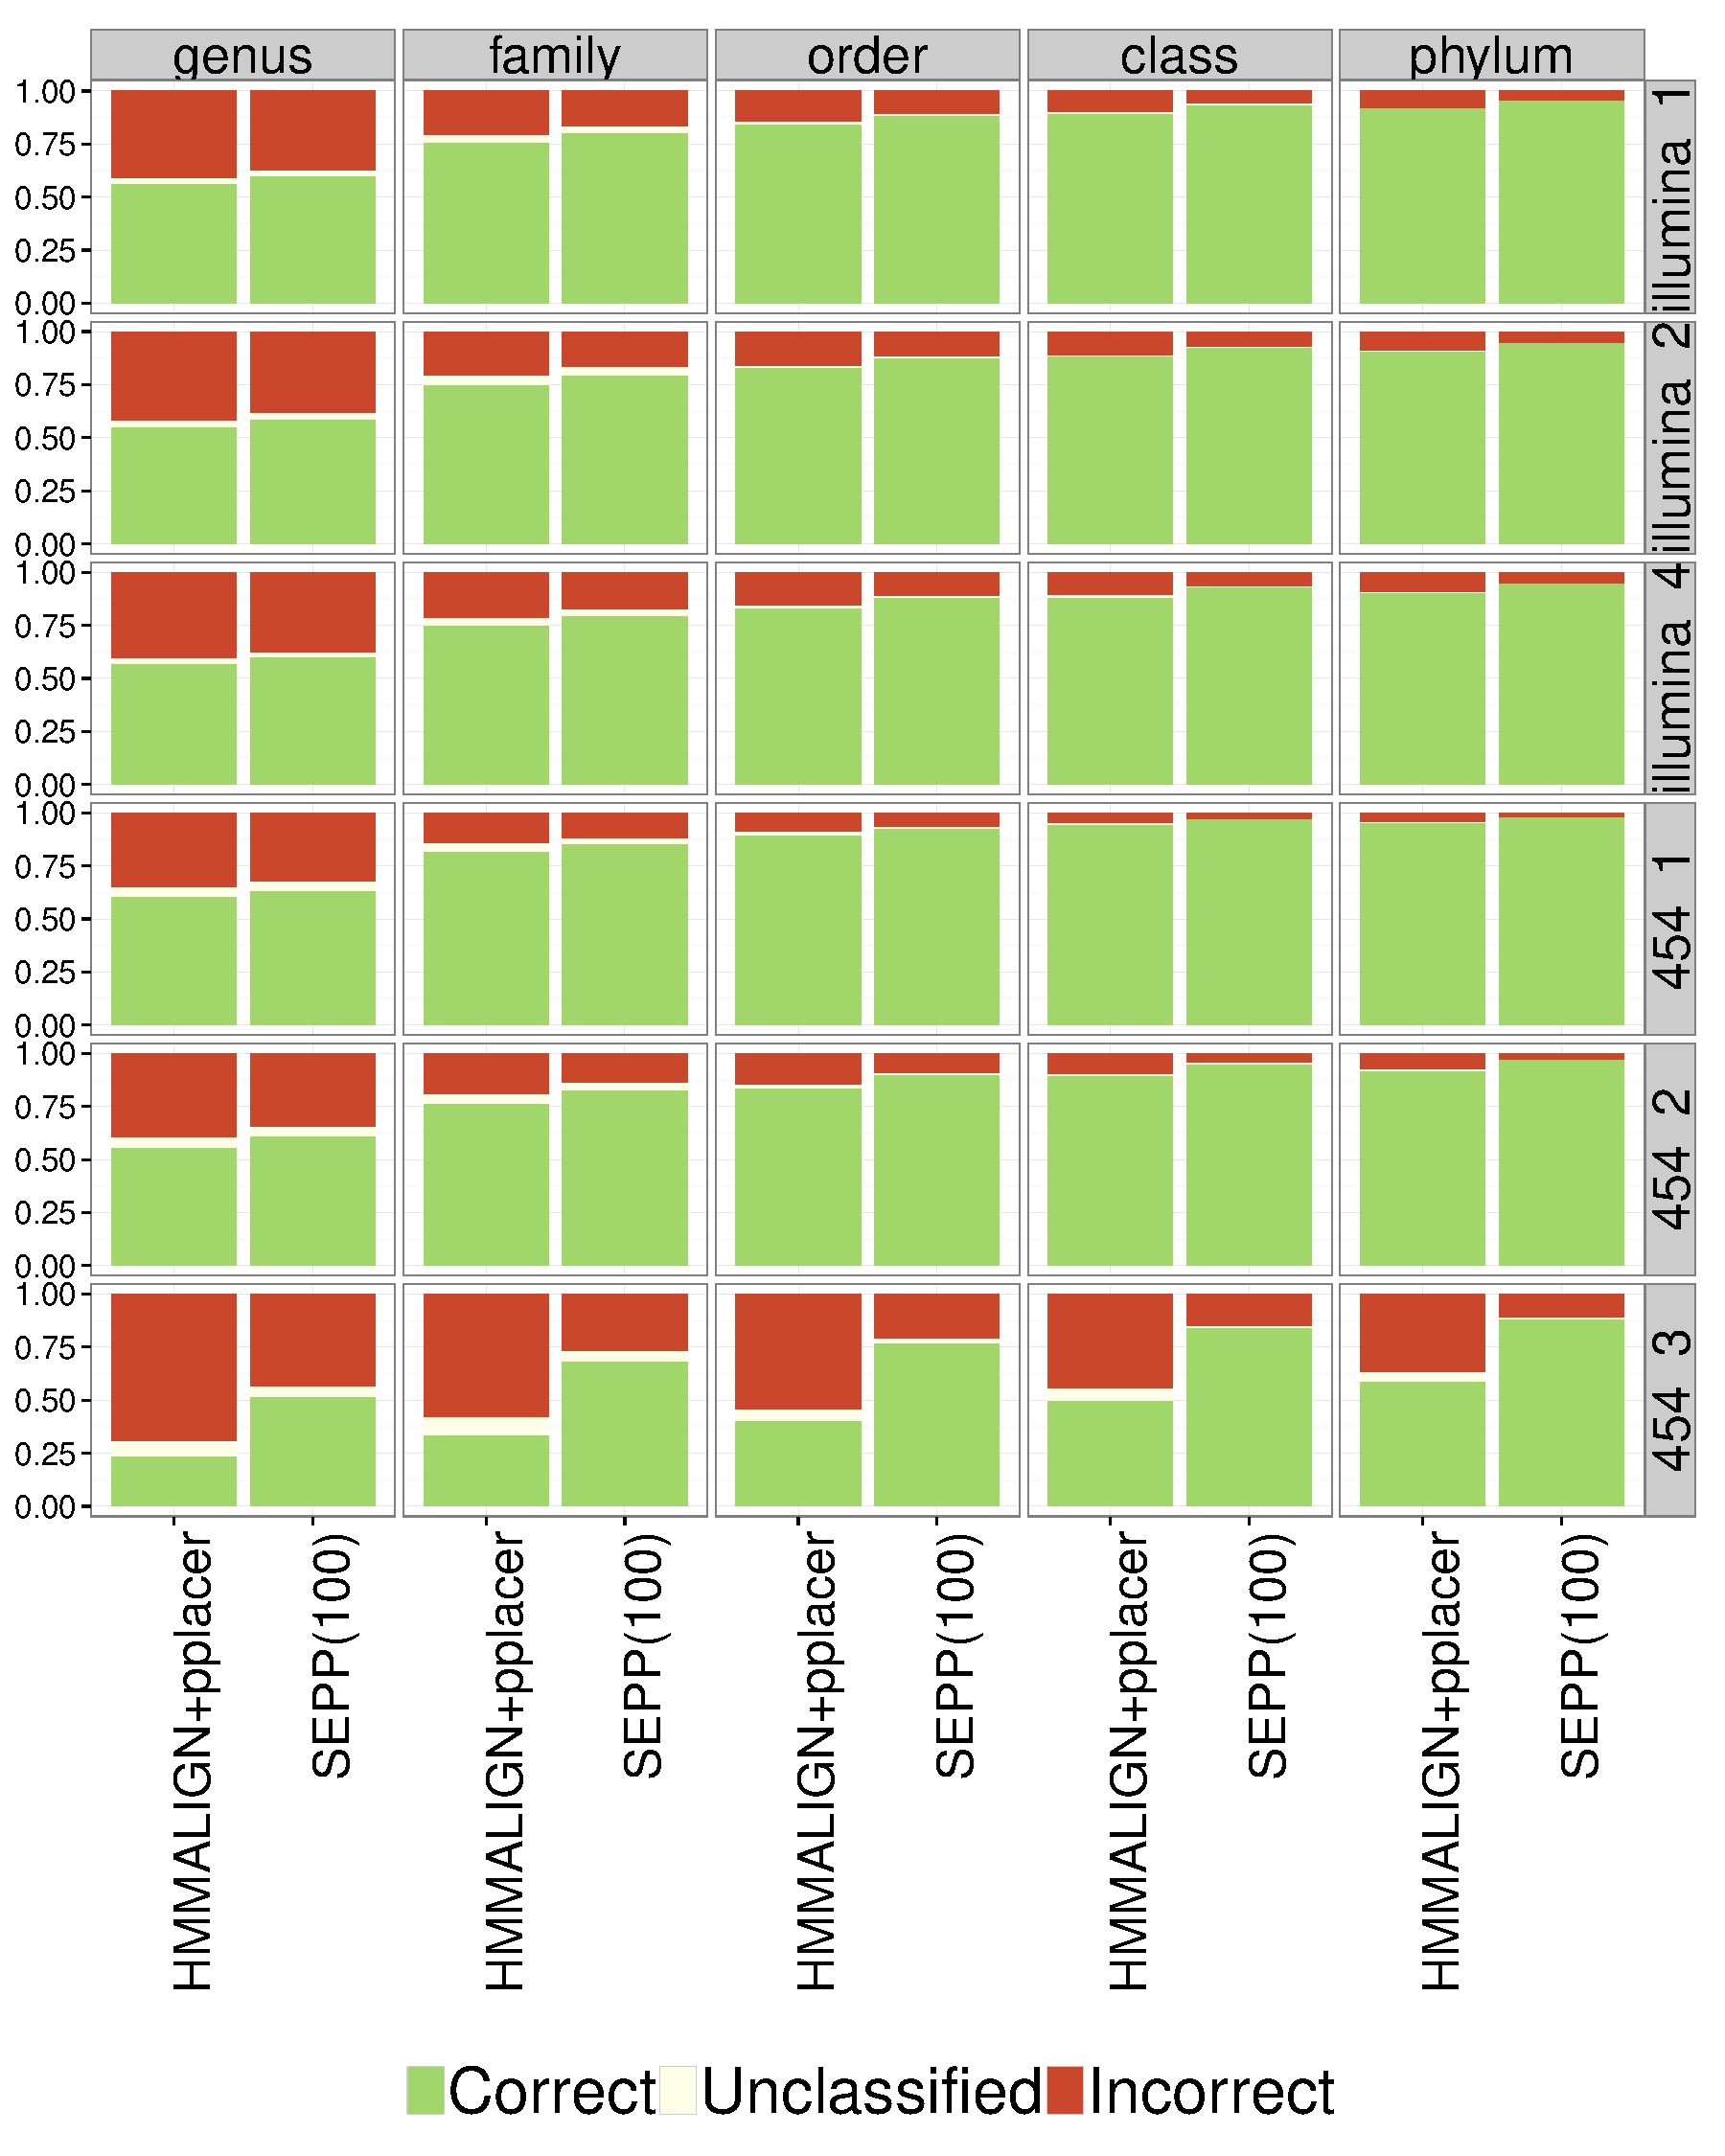
\includegraphics[scale=0.4]{{tipp/sepp.species}.pdf}}
% \end{center}
% \caption[Comparing SEPP and HMMALIGN+pplacer for taxonomic identification]{\label{tipp:preliminary_sepp} Leave-species-out experiments comparing SEPP and HMMALIGN+pplacer taxonomic classification accuracy on the rpsB gene under sequences simulated under different error model conditions.  Fragments were simulated with either Illumina-like or 454-like errors, and with varying rates of error.  Models denoted with a ``1'' have the lowest rates of error, and models with a ``3'' or ``4'' have the highest rates of error.  SEPP is run using a alignment decomposition size of 100 and placing on the entire backbone tree.}
% \end{figure}

%Taxon identification methods only classify a
%subset of the fragments (some correctly and some incorrectly), and
%will leave some fragments unclassified at each taxonomic level.
%Therefore, evaluations of taxonomic classification methods
%consider the percent of fragments classified
%at each rank correctly, incorrectly, or unclassified.  

%However, accurate classifications of just the fragments matching
%marker genes is sufficient for many purposes.
%For example, most culture-independent
%studies of microbial communities have relied on the
%analysis of the 16S rRNA gene.
%These studies, generating broad taxonomic profiles of the
%communities being studied, have been the basis for
%many important discoveries in microbial ecology and
%biomedicine  \cite{Turnbaugh2009}. % Alternative: Aagaard2012, Belda-Ferre2012
%In addition, 
%taxon identification methods should accurately label
%sequences already found in public databases, but should also provide accurate
%guesses on the taxonomy of sequences that are only distantly related
%to known sequences.  In fact, identifying novel organisms or taxonomic
%clades is an important focus of recent studies~\cite{eisen} and taxon
%identification software should be able to accurately identify putative
%novel organisms.  


% We have developed TIPP, a new method for taxon
% identification and phylogenetic profiling.
% TIPP is a marker-based method, but can be used to
% characterize any sequence matching any gene for which
% a dense enough sample of full-length sequences are
% available. In this paper, we explore TIPP using the
% Metaphyler's collection of 30 marker genes.

%\subsection{Ultra-large alignment estimation}\label{back:ultra_large}
